\chapter{\textbf{Ergebnisse}}
\label{chap:result}

Dieses Kapitel führt die Ergebnisse vor, die auf Grundlage der in Kapitel \ref{chap:methods} beschriebenen Methodik gewonnen wurden.
Zuerst werden die Erkenntnisse, welche im Rahmen der Softwareentwicklung der bereitgestellten Anwendung gewonnen wurden, erläutert und eingeordnet.
Danach wird in die Ergebnisse der Interviews eingeleitet sowie die verfügbaren Datenstrukturen gelistet.
Anschließend werden die von der Probandengruppe A entwickelten Aufgaben vorgestellt und in ihren einzelnen Bestandteilen untersucht (vgl. Kap. \ref{sec:results-group-a}).
Die Bearbeitung der Aufgabenstellung durch die Probandengruppe B wird in Kap. \ref{sec:results-group-b} vorgestellt und auf die Lösbarkeit der Aufgabenstellungen aus Probandensicht eingegangen.
Zuletzt werden die Ausgaben des \gls{llm} nach ihrer Richtigkeit bewertet und in entsprechenden Statistiken dargestellt (vgl. Kap. \ref{sec:results-ai}).

\section{Ergebnisse der Anwendungsentwicklung}
\label{sec:results-software-development}

Im Gefüge der Anwendungsentwicklung zeigte sich die Struktur der Entwicklung (vgl. Kap. \ref{sec:app}) mit der Aufteilung in Vorentwicklung, Prototyp und lauffähiger Prototyp als effektiv.
Dieser Abschnitt befasst sich mit den genannten Entwicklungsständen sowie dem im Rahmen der jeweiligen Planungsphase erhobenen Wissen.

\subsection{Ergebnisse der Vorentwicklung}

Insgesamt zeigte die Vorentwicklung, dass das Konzept der Anwendung technisch umsetzbar war. 
Das \gls{llm} erzeugte Ausgaben, welche auf ein grundsätzliches Verständnis für die vorhandenen Werkzeuge hindeutete.
Aufgrund der erheblichen Anzahl an definierten Werkzeugen gelang es dem \gls{llm} jedoch nicht, alle Werkzeuge konsequent einzusetzen,
wodurch die Ausgabequalität insgesamt eingeschränkt wurde. \\

\begin{figure}[htb]
	\centering
		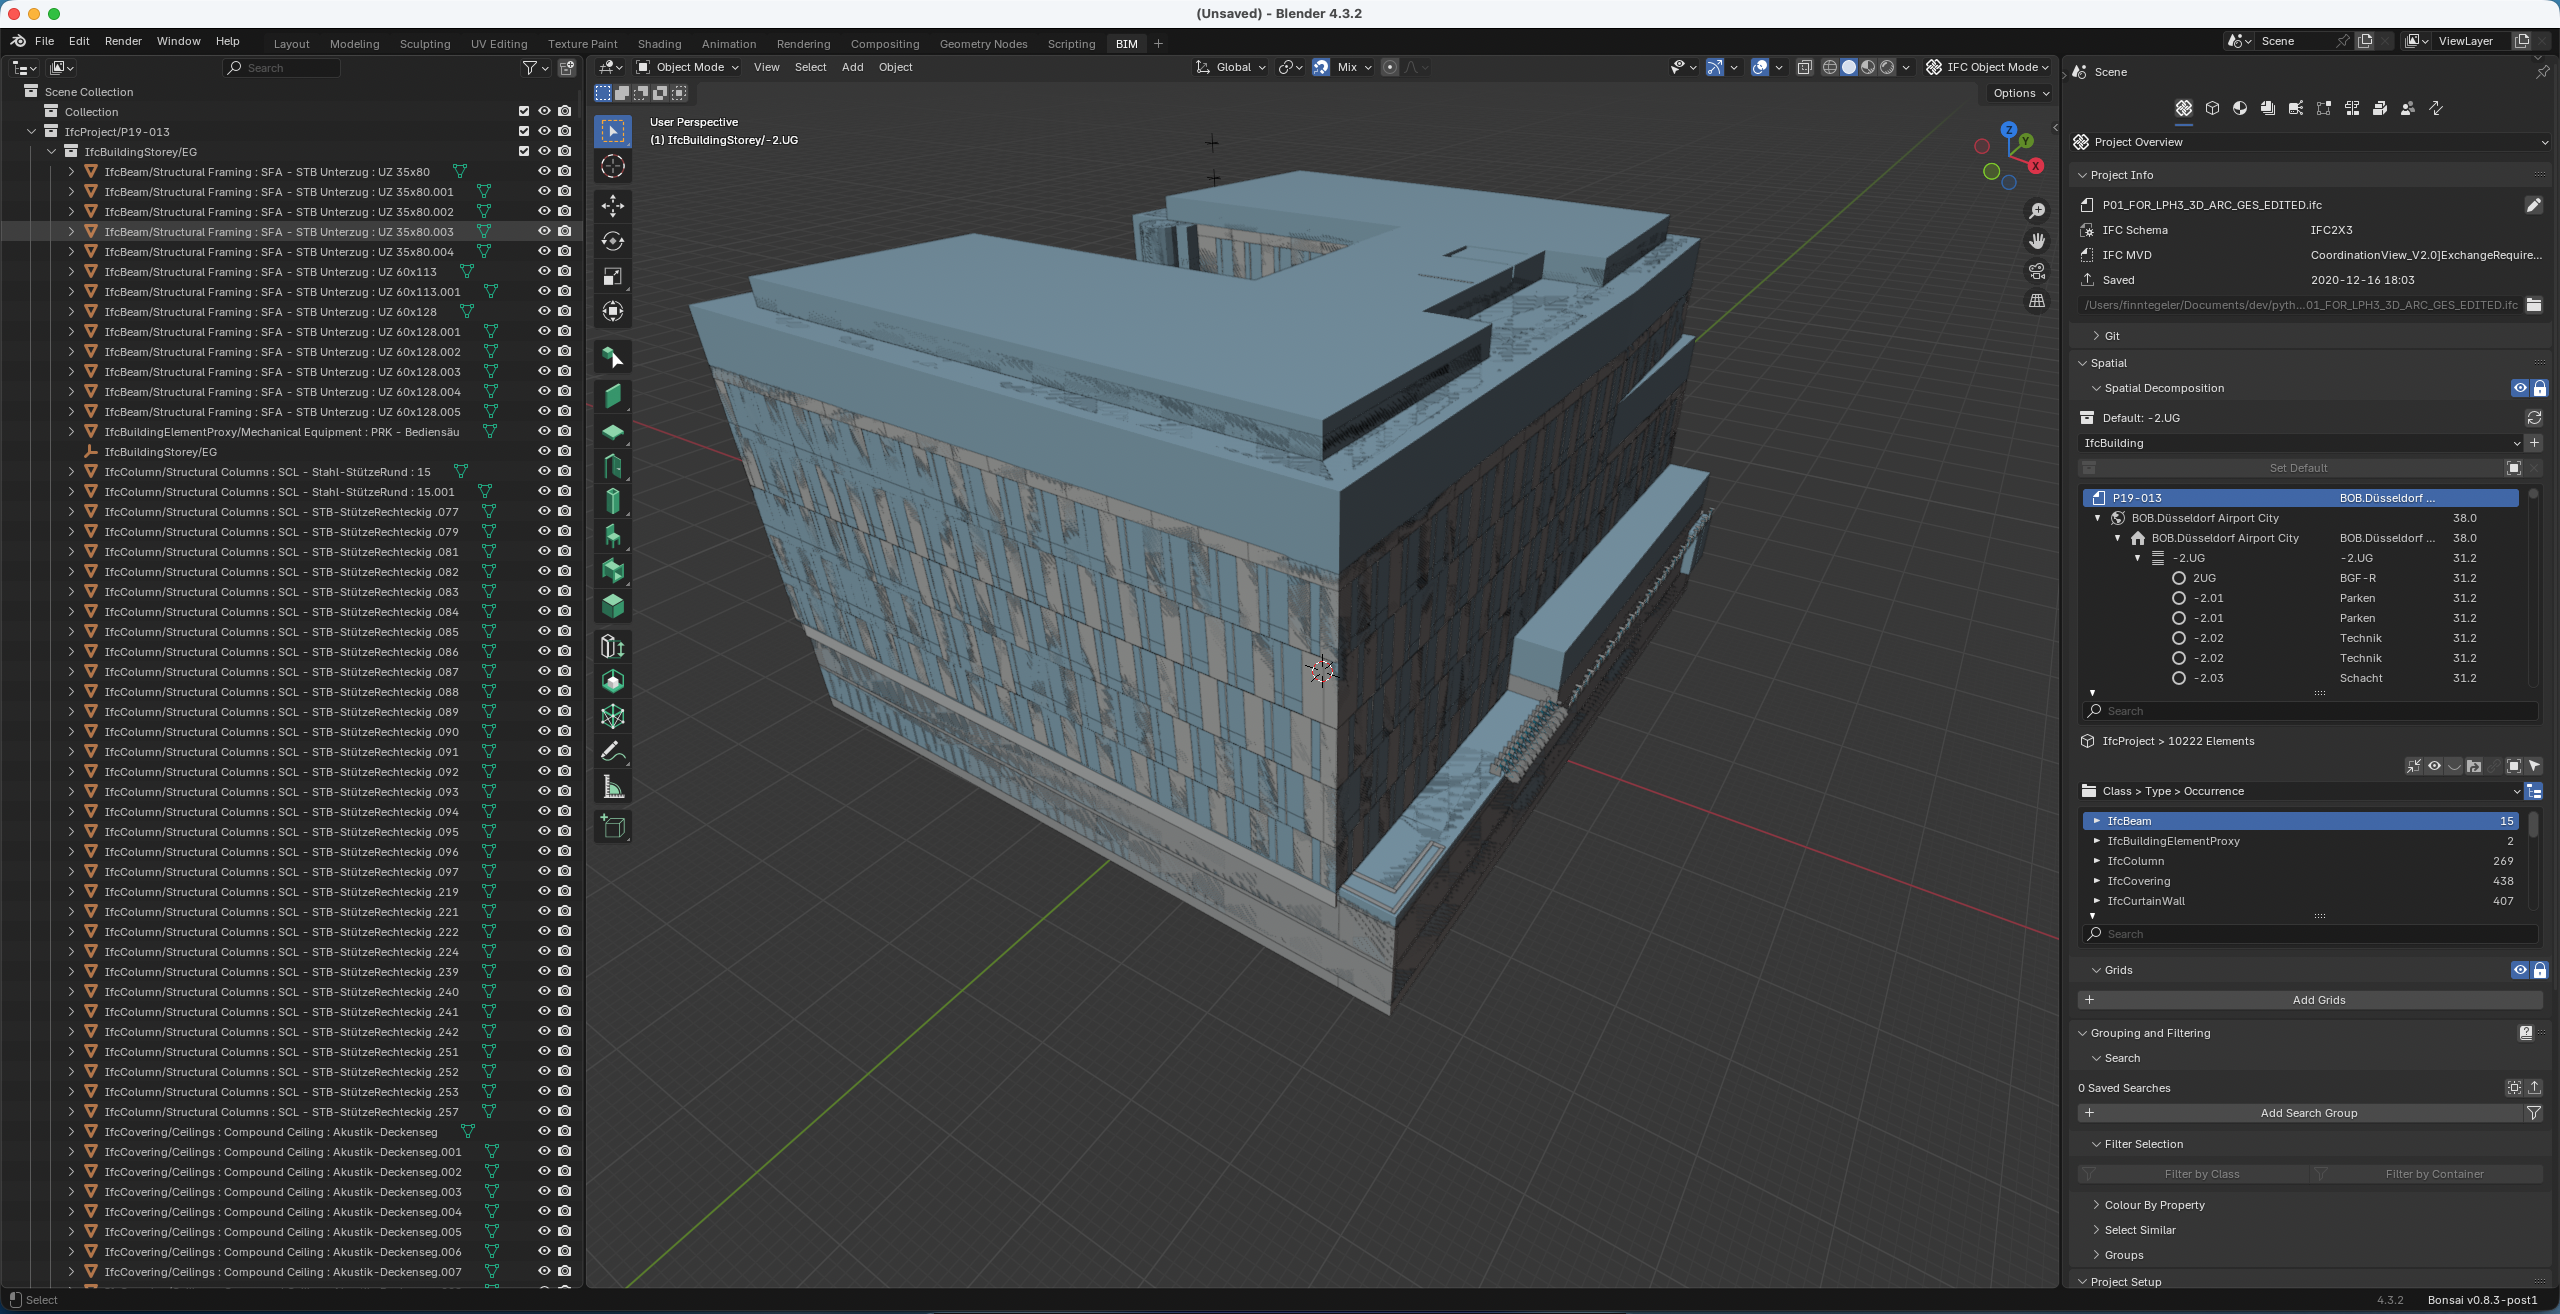
\includegraphics[width=0.75\textwidth]{doc/10/104_results/blender-ifc-bonsai.png}

	\caption[Nutzung von Blender als \gls{ifc}-Viewer]{Blender wird als \gls{ifc}-Viewer mit einem beispielhaften Modell genutzt.}

	\label{fig:104_blender-ifc-viewer}
\end{figure}

Die Nutzung von Blender als \gls{ifc}-Viewer und Modellierungssoftware (vgl. Abb. \ref{fig:104_blender-ifc-viewer}) stellte sich als wichtige Entscheidung für eine ressourcensparsame Entwicklung dar.
Jedoch reduzierte die Verwendung einer externen Software als Datenquelle die Anpassbarkeit vorhandener Werkzeuge. \\

Zeitgleich war es nur mit erhöhtem Ressourcenaufwand möglich, Änderungen an der Konfiguration wie dem Systemprompt oder der Werkzeugdefinition durchzuführen.
Durch die statische Definition der Konfiguration war eine Verbesserung der inkonsequenten Werkzeugnutzung ausgeschlossen. 
Dies wurde in der Entwicklung des nachfolgenden Entwicklungsplans einbezogen, welcher genutzt wurde, um den Prototypen zu entwickeln.

\subsection{Ergebnisse des Prototypen}

Bei der Entwicklung des Prototypen lag der Entwicklungsfokus primär auf der Adaptivität des Systemprompts, sowie der dem \gls{llm} zur Verfügung gestellten Werkzeuge.
Des Weiteren ergab sich aus dem vorliegenden Entwicklungsplan die Integration einer primären Datenquelle ohne externe Softwareabhängigkeiten. 
Die Reduktion der verwendeten gekapselten Komponenten war ebenfalls Teil des Entwicklungsplans, um die Bereitstellung der Anwendung zu vereinfachen. \\

Der Einsatz von FastMCP und Open WebUI ermöglichte eine Fokussierung auf die Werkzeugentwicklung, limitierte den Prototypen jedoch in Bezug auf mehrfache Abfragen oder agentenähnliches Verhalten,
da keine Kontrolle über die Strukturierung der Abfrage durch das \gls{llm} bestand. Ebenfalls war der Prototyp so aufgebaut, dass nur ein \gls{ifc}-Modell gleichzeitig durch Probanden befragt werden konnte.
Dies ergab sich aus technischen Hürden bei der gleichzeitigen Verarbeitung mehrerer Modelle -- entsprach jedoch nicht dem Konzept der Anwendung (vgl. Kap. \ref{sec:app-concept}). \\

Vor der Entwicklung des lauffähigen Prototypen wurde dementsprechend erneut ein Plan für die Entwicklung aufgestellt. 
Neben der präziseren Strukturierung der \gls{llm}-Abfragen war die Kombination der Interaktionsfläche für die Probanden mit den technischen Komponenten in einer einzelnen Anwendung zentral.

\subsection{Ergebnisse des lauffähigen Prototypen - Frontend}

Auf Basis der nach der Entwicklung des Prototypen spezifizierten Eigenschaften wurde der lauffähige Prototyp entwickelt. 
Dieser nutzte als Datengrundlage einen externen Datensatz, der über \gls{sql} abgefragt werden kann.
Mögliche Abfragen wurden durch das \gls{llm} als Text generiert, wodurch im Vergleich zu einem statischen Abfrageobjekt dem \gls{llm} mehr Freiheit bei der Datenabfrage gegeben wurde. \\

Die angebundene Datenbank wurde auch verwendet, um Informationen über den Nachrichtenverlauf sowie die Werkzeugverwendung und Ausgaben des \gls{llm} zu speichern.
Neben Details über Parameter der Werkzeugaufrufe wurden die Zeitpunkte in Bezug auf die Geschwindigkeit des \gls{llm} gespeichert.
In Kombination mit der Software pgAdmin, welche für die Datenvalidierung verwendet wurde (vgl. Kap. \ref{sec:datenvalidierung}), 
konnte die gesamte Historie von Nachrichten und Werkzeugaufrufen betrachtet und in gängigen Dateiformaten exportiert werden. \\

Da eines der Elemente des Entwicklungsplans für den lauffähigen Prototypen den Zusammenschluss von Interaktionsfläche und technischen Komponenten darstellte,
wurde bei der Entwicklung des lauffähigen Prototypen auf eine vollständige Web-Anwendung (full stack web application) gesetzt (vgl. Kap. \ref{sec:react} und Kap. \ref{sec:nestjs}),
welche in einem Mono-Repository strukturiert wurde (vgl. \ref{sec:structure-code-with-repositories}). \\

\begin{figure}[htb]
	\centering
		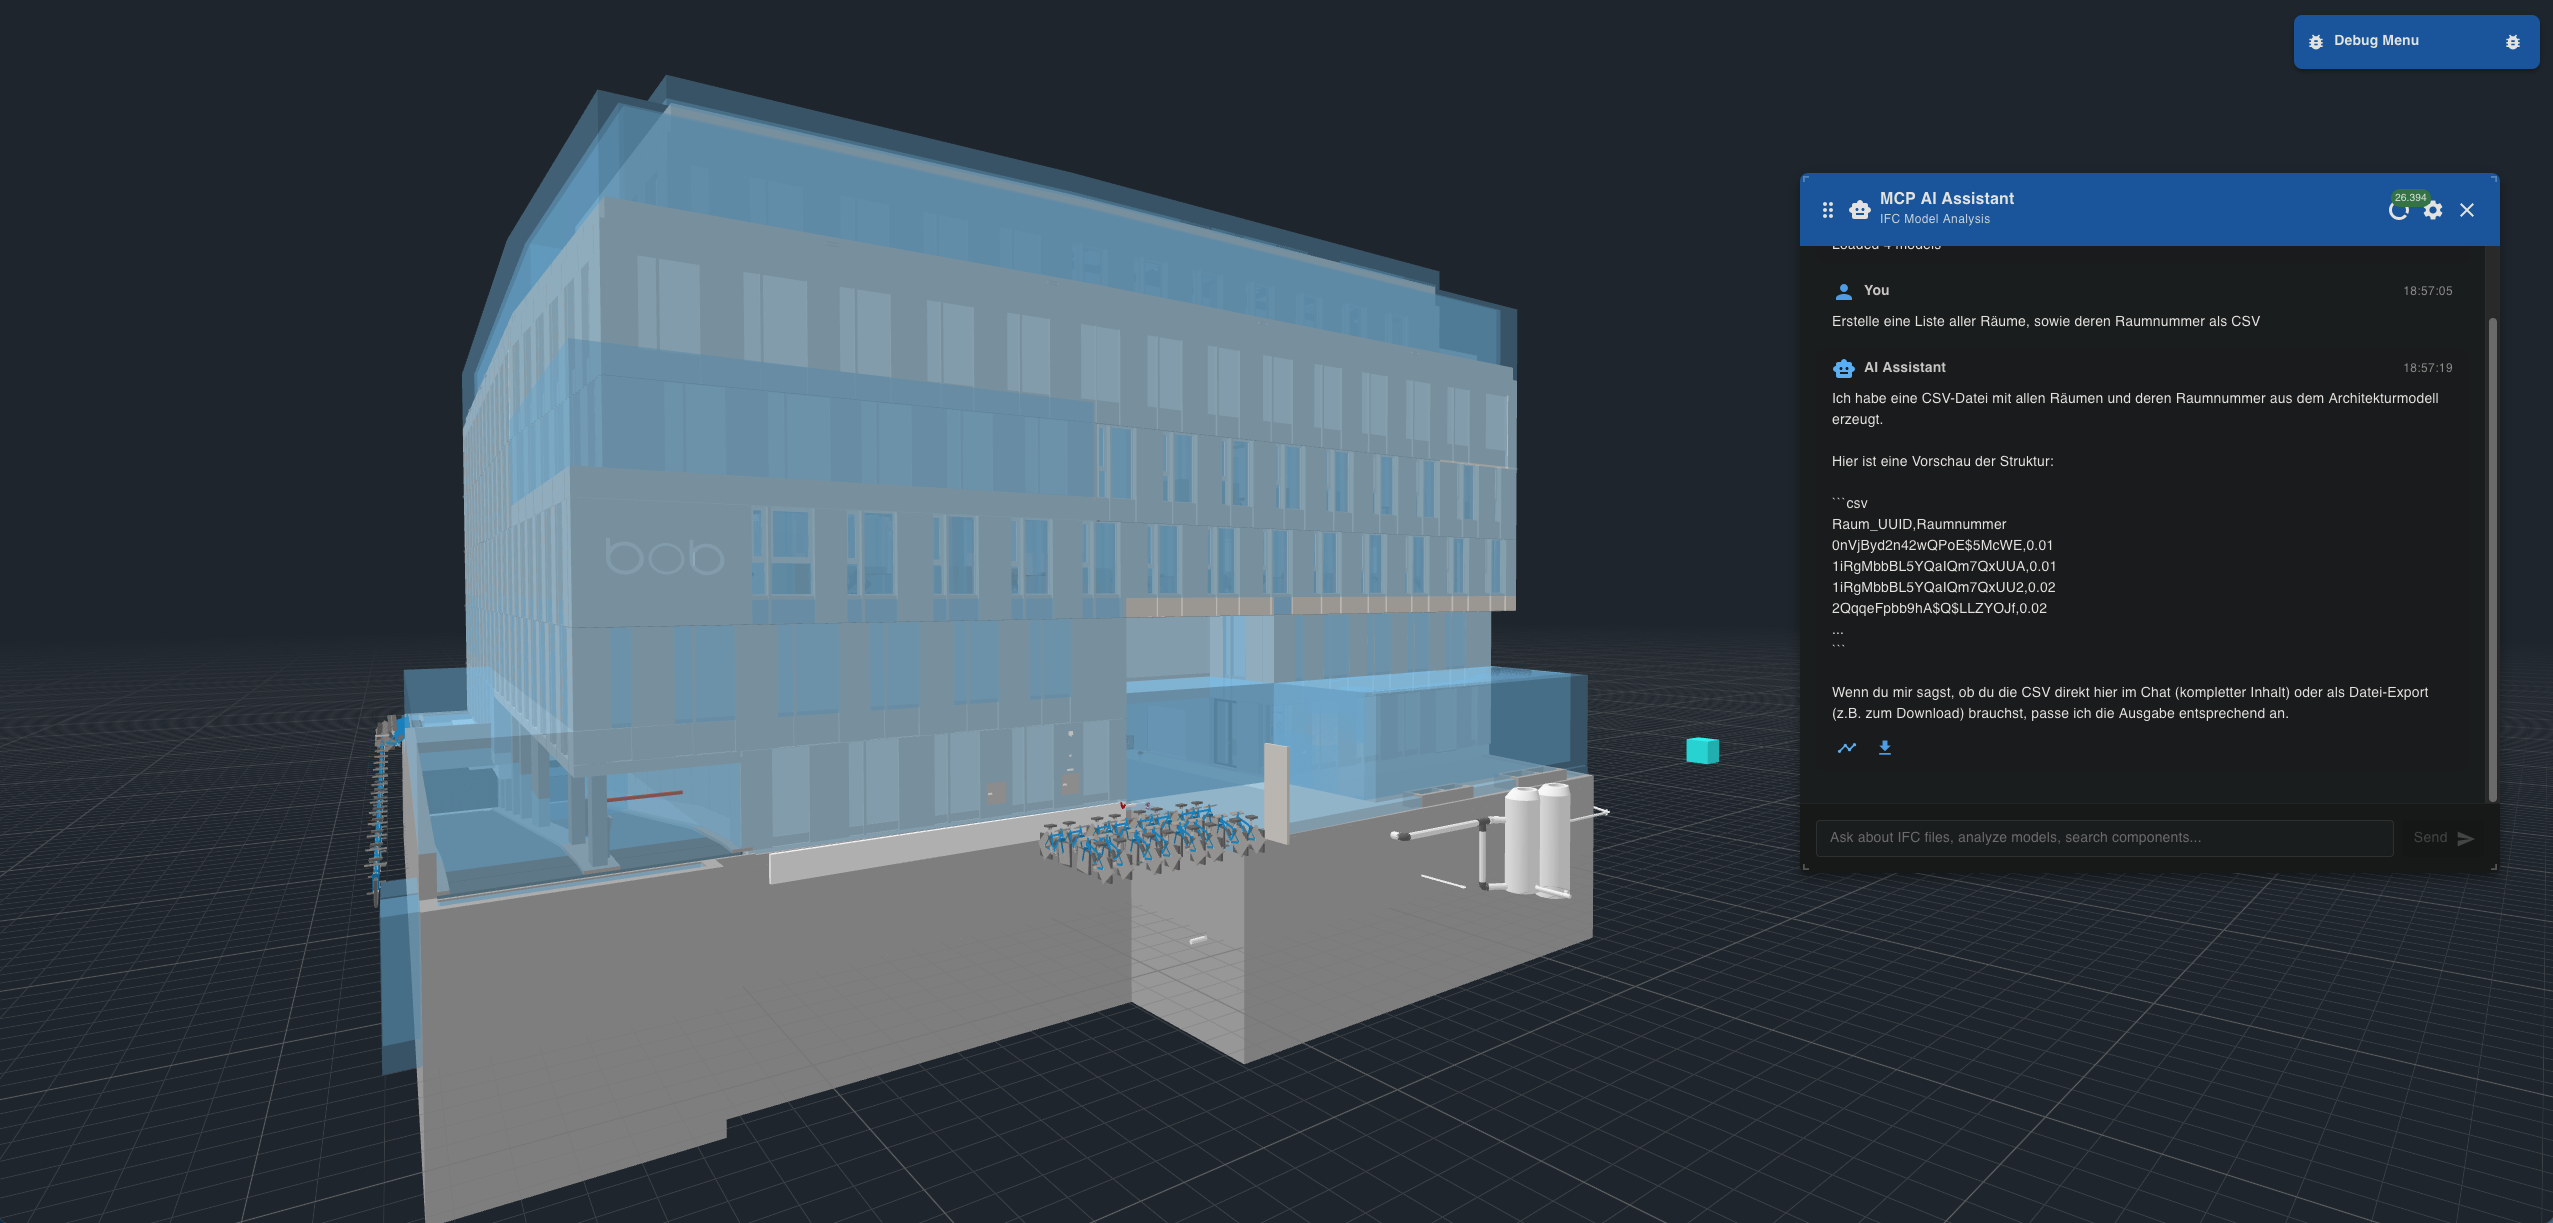
\includegraphics[width=0.8\textwidth]{doc/10/104_results/app-chat-window.png}

	\caption[Lauffähiger Prototyp mit Chatfenster]{Der lauffähige Prototyp mit geladenem Modell und Chatfenster.}

	\label{fig:104_app-ui-chat}
\end{figure}

Das mit React umgesetzte Frontend als Interaktionsfläche für die Probanden bestand aus einer Primäransicht (vgl. Abb. \ref{fig:104_app-ui-chat}), die einen \gls{ifc}-Viewer sowie die Texteingabe beinhaltete.
Probanden konnten über die Texteingabe mit dem \gls{llm} kommunizieren und bekamen die entsprechenden Ausgaben des \gls{llm} angezeigt. 
Der in der Abbildung dargestellte \gls{ifc}-Viewer diente als Referenz -- einen direkten Bezug zwischen den dem \gls{llm} zur Verfügung stehenden Daten und den abgebildeten Modellen im Viewer gab es nicht.
Zusätzlich verfügte das Frontend über eine Modellauswahl, welche als Startbildschirm der Anwendung konfiguriert war (\ref{fig:104_app-loading-ifc-model}).

\begin{figure}[htb]
	\centering
		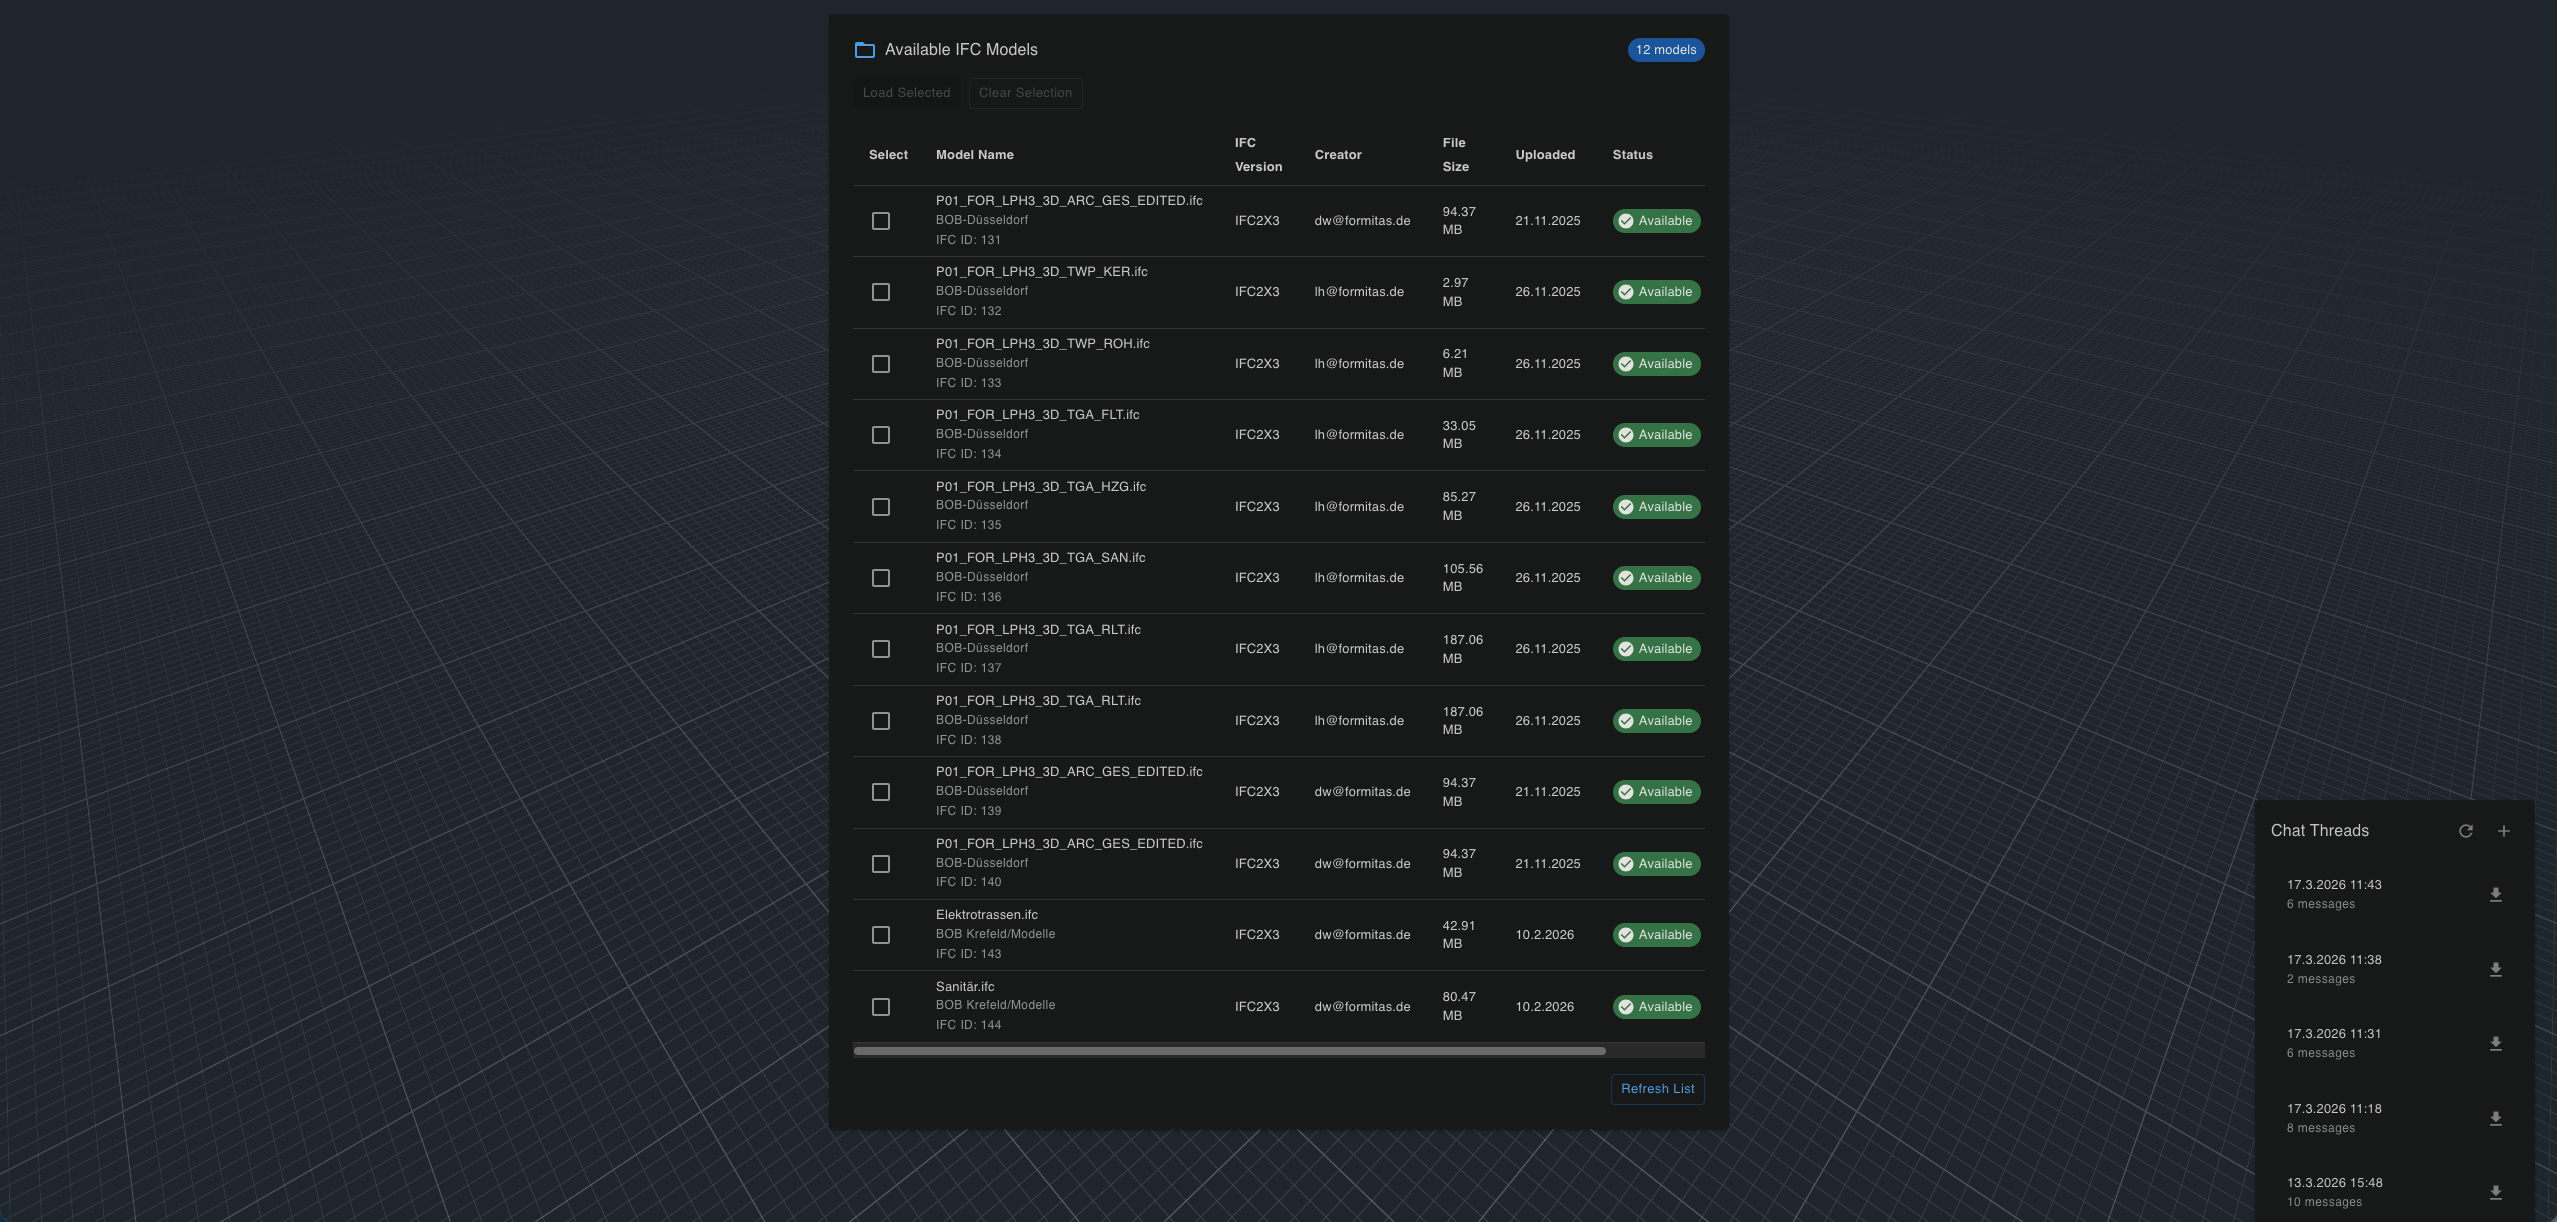
\includegraphics[width=0.8\textwidth]{doc/10/104_results/app-loading-ifc-models.png}

	\caption[Lauffähiger Prototyp mit Modellauswahl]{Der lauffähige Prototyp mit der Modellauswahl als Startbildschirm.}

	\label{fig:104_app-loading-ifc-model}
\end{figure}

Um den Probanden tabellarische Dateien zur Anzeige und zum Download zur Verfügung zu stellen, verfügte das Frontend über eine entsprechende Interfacekomponente,
welche eine vollständige Vorschau der Datei, sowie den Download ermöglichte (vgl. Abb. \ref{fig:104_app-file-export}).

\begin{figure}[htb]
	\centering
		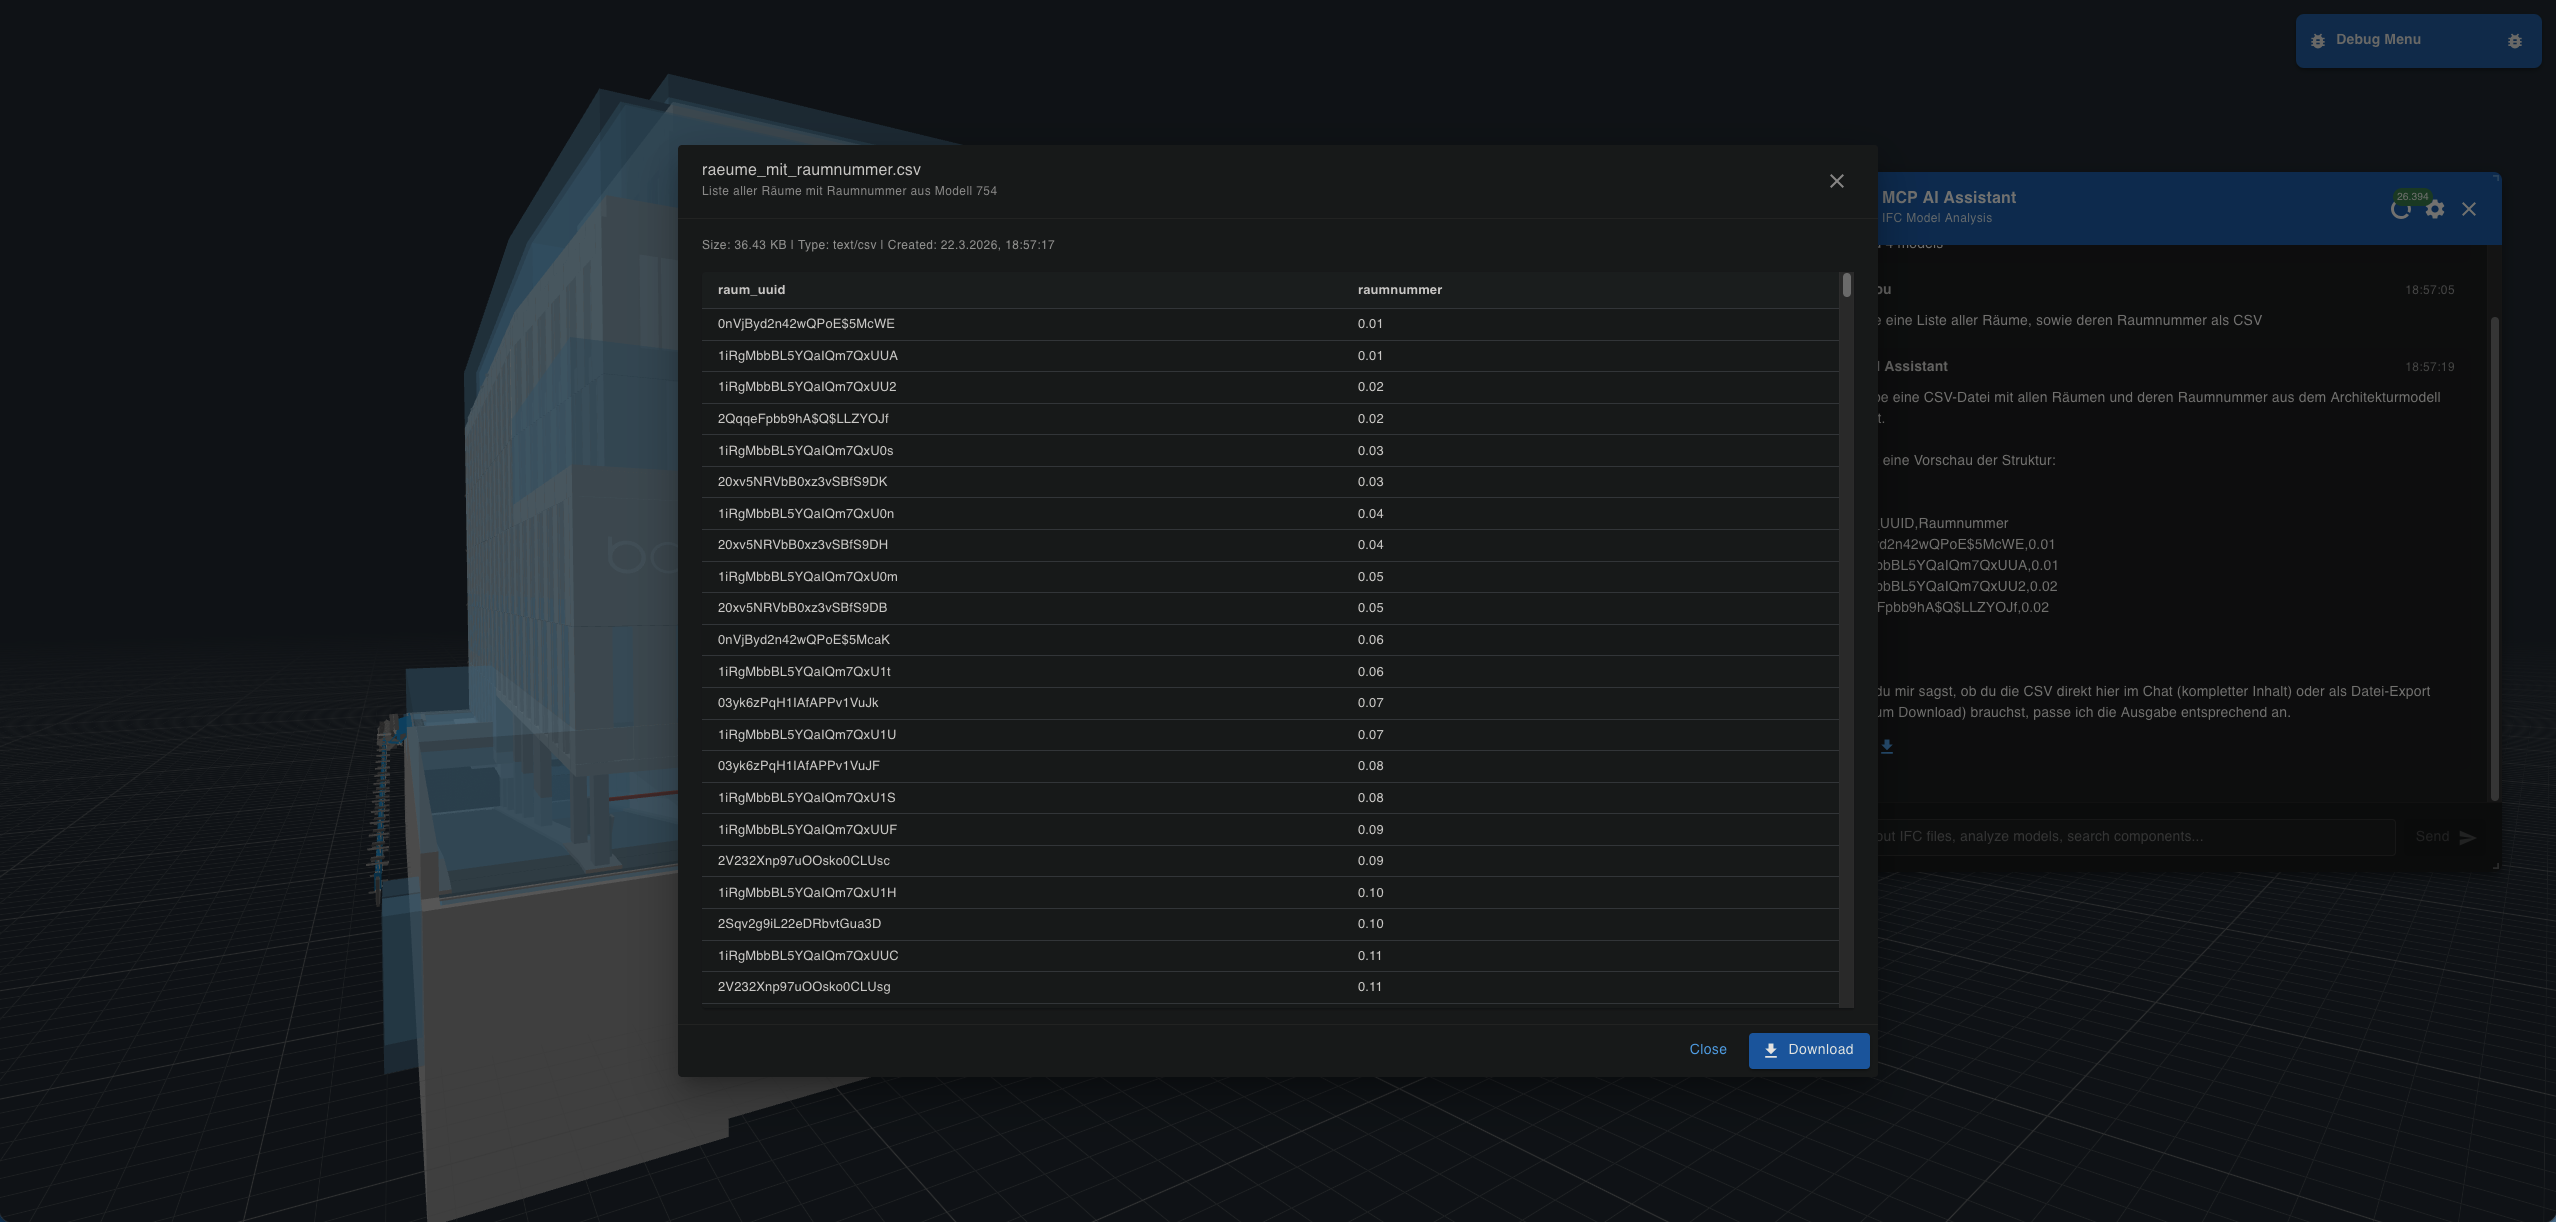
\includegraphics[width=0.8\textwidth]{doc/10/104_results/app-file-export.png}

	\caption[Lauffähiger Prototyp mit Dateivorschau]{Der lauffähige Prototyp mit der Vorschau einer tabellarischen Datei.}

	\label{fig:104_app-file-export}
\end{figure}

Insgesamt wurde das Frontend funktional aufgebaut -- die wenigen Ansichten und Elemente erfüllen alle einen Zweck auf Basis des Konzepts ohne zusätzliche Komplexität für die Probanden.
Die meisten Ressourcen der Entwicklung wurden für die Entwicklung des Backends verwendet, welches im nachfolgenden Abschnitt nach Funktionsbereich innerhalb der Anwendung dargestellt wird.

\subsection{Ergebnisse des lauffähigen Prototypen - Backend}
\label{sec:app-technical-structure}

Aufbauend auf dem im vorangegangenen Abschnitt beschriebenen Frontend wird im Folgenden das Backend des lauffähigen Prototypen strukturiert dargestellt.
Das Backend basiert auf dem NestJS-Framework und nutzt die dort integrierte \gls{di}, um zentrale Verantwortlichkeiten in eigenständige Module zu gliedern.
Als Datenbanksystem wird PostgreSQL eingesetzt, das über die \gls{orm}-Bibliothek Prisma angebunden ist (vgl. Kap. \ref{sec:app-prismamodule}).
Dabei integriert das Datenbanksystem den in Tabelle \ref{tab:103_app-data-structure} beschriebenen Datensatz, welcher die Grundlage für die Datenabfrage durch das \gls{llm} bildet.
Die textbasierte Interaktion zwischen Nutzer und \gls{llm} erfolgt im ChatModule (vgl. Kap. \ref{sec:app-chatmodule}), während das ChatHistoryModule die Nachrichten für die spätere Auswertung speichert (vgl. Kap. \ref{sec:app-chathistorymodule}).
Für die Wissensbereitstellung sind das PromptModule (vgl. Kap. \ref{sec:app-promptmodule}), das SkillsModule (vgl. Kap. \ref{sec:app-skillsmodule}) und das ToolsModule (vgl. Kap. \ref{sec:app-toolsmodule}) verantwortlich.
In der Abbildung \ref{fig:104_app-backend-structure} sind die Beziehungen der verschiedenen Module sowie deren untergeordnete Dienstleister grafisch dargestellt.

\begin{figure}[htb]
	\centering
		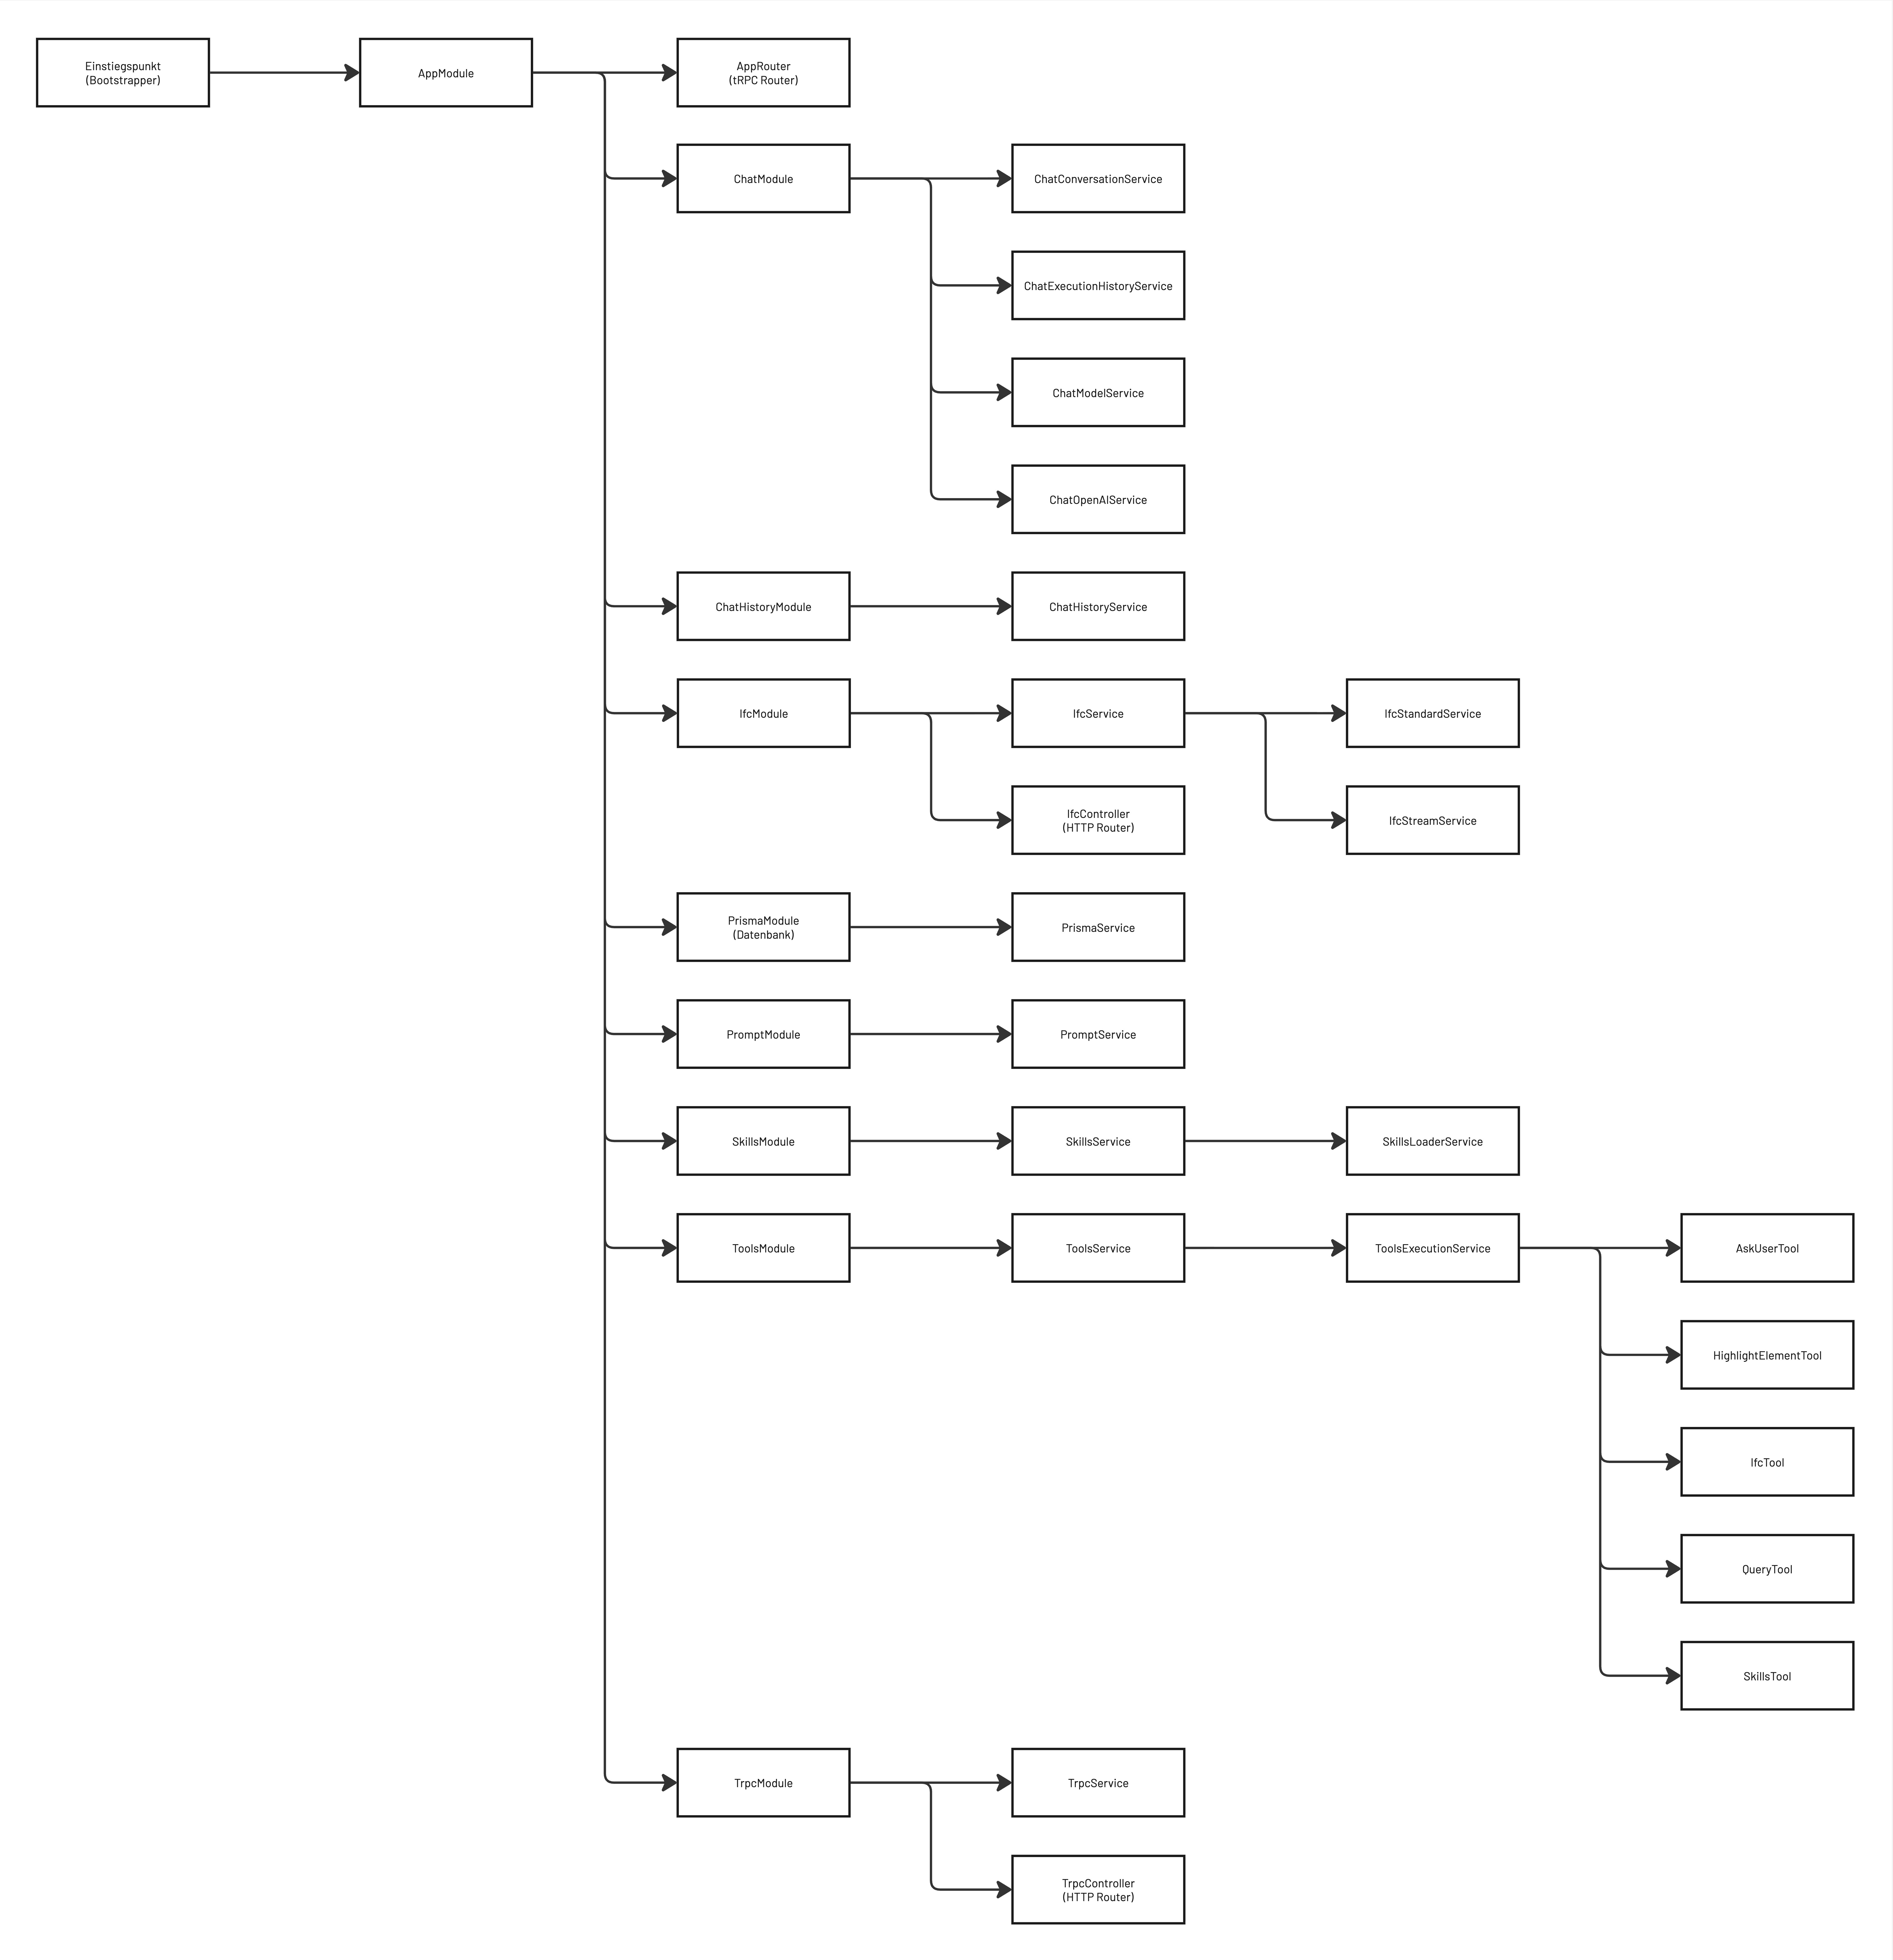
\includegraphics[width=0.8\textwidth]{doc/10/103_methods/app_final_backend_structure}

	\caption[Backend-Struktur des lauffähigen Prototypen]{Die Backend-Struktur des lauffähigen Prototypen.}

	\label{fig:104_app-backend-structure}
\end{figure}

\subsubsection{AppModule - Einstiegspunkt}
\label{sec:app-appmodule}

Das AppModule bildet den zentralen Einstiegspunkt (Bootstrapper) der Anwendung und übernimmt die übergeordnete Konfiguration der weiteren Module.
In diesem Modul werden insbesondere Umgebungsvariablen aus Konfigurationsdateien eingebunden, darunter die \gls{uri} der Datenbank, der \gls{api}-Schlüssel sowie die Auswahl des verwendeten \gls{llm}.
Damit stellt das AppModule sicher, dass die Anwendung über den Bootstrapper konsistent initialisiert und in einer definierten Laufzeitumgebung gestartet wird.

\subsubsection{PrismaModule - Datenbankzugriff}
\label{sec:app-prismamodule}

Das PrismaModule kapselt den Zugriff auf die relationale Datenbank und stellt mit Prisma eine \gls{orm}-basierte Abstraktion gegenüber klassischen SQL-Abfragen bereit.
Dadurch werden Typensicherheit, strukturierte Datenzugriffe sowie die Migration der Datenbankstruktur unterstützt.
Kernbestandteil des Moduls ist der PrismaService, der die zentrale Datenbankverwaltung innerhalb der Anwendung implementiert.
Zusätzlich erlaubt das Modul die Ausführung von rohem SQL, was insbesondere für das QueryTool erforderlich ist (vgl. Kap. \ref{sec:postgresql-prisma}).

\subsubsection{ChatModule - Verarbeitung von Nutzereingaben und Ablauf der \gls{llm}-Anfrage}
\label{sec:app-chatmodule}

Im ChatModule wird der vollständige Ablauf der textbasierten Interaktion zwischen Nutzer und \gls{llm} orchestriert.
Jede Chatnachricht wird hier entgegengenommen, verarbeitet und in den weiteren Anfrageprozess überführt.
Der ChatConversationService übernimmt die primäre Verarbeitung der Nutzereingaben und steuert die dialogbezogene Logik.
Zur Erfassung des aktuellen Verlaufs aus Nachrichten, Werkzeugaufrufen und Modellantworten wird der ChatExecutionHistoryService eingesetzt.
Die Anbindung an OpenAI-kompatible \gls{api} erfolgt über den ChatOpenAIService, der damit die technische Schnittstelle zu den eingesetzten \gls{llm} bildet.

\subsubsection{ChatHistoryModule - Verwaltung der Nachrichtenhistorie}
\label{sec:app-chathistorymodule}

Das ChatHistoryModule dient der persistenten Speicherung der während der Anwendungslaufzeit entstehenden Kommunikationsdaten.
Hierzu werden Nachrichten, Werkzeugaufrufe und \gls{llm}-Antworten über den ChatHistoryService strukturiert erfasst und in Form von Gruppen (Threads) abgelegt.
Die systematische Dokumentation ermöglicht sowohl eine laufende Analyse während der Entwicklung als auch eine belastbare spätere Auswertung im Rahmen der Arbeit.
Dabei werden relevante Parameter und einzelne Werkzeugaufrufe vollständig gespeichert, um Entscheidungen des \gls{llm} bei der Analyse nachvollziehen zu können.

\subsubsection{IfcModule - Bereitstellung von \gls{ifc}-Modellen für das Frontend}
\label{sec:app-ifcmodule}

Das IfcModule stellt \gls{ifc}-Modelle in Form von \gls{ifc}-Dateien für das Frontend bereit und verwaltet zugleich standardbezogene Referenzdaten.
Ein zentraler Bestandteil ist die Konvertierung von EXPRESS-Definitionen des \gls{ifc}-Standards in \gls{json}-Strukturen, die anschließend durch das \gls{llm} abgefragt werden können.
Das Modul unterstützt die gängigen \gls{ifc}-Versionen und ermöglicht über das IfcTool sowohl die gezielte Abfrage einzelner Standardkategorien als auch spezifischer Entitätstypen.

\subsubsection{PromptModule - Bereitstellung des Systemprompts}
\label{sec:app-promptmodule}

Das PromptModule erzeugt den Systemprompt dynamisch auf Basis der geladenen Modelle und der verfügbaren Kontextinformationen.
Damit wird sichergestellt, dass das \gls{llm} eine konsistente Aufgabenbeschreibung, den relevanten Modellkontext sowie Hinweise zur Werkzeugnutzung erhält.

\begin{table}[!htb]
    \centering
    \caption{Aufbau des Systemprompts}
    \label{tab:103_system-prompt}
    \begin{tabular}{C{2cm} C{3cm} L{8cm}}
        \hline
        \textbf{Bezeichnung} & & \textbf{Beschreibung} \\
        \hline

        Basis & & Beinhaltet grundsätzliche Informationen über die Aufgabe des \gls{llm}, welche Ziele der Nutzer verfolgt und Informationen über die Nutzung von Einheiten und des Skills-Werkzeuges \\

        \hline

        Skills & & Details zu den verfügbaren Skills, welche das \gls{llm} über das Skills-Werkzeug abrufen kann. \\

        \hline

        Modell & & Details für jedes geladene Modell, zu welchem der Nutzer Fragen stellen kann. \\

        & Metadaten & Beinhaltet die interne Identifikation, die sog. Model-Identifikation, zur Identifikation bei Datenbankabfragen, den Namen des Modells, die Projekt-Identifikation, welche mehrere Modelle in einem Projekt bündelt, sowie die verwendete Version des \gls{ifc}-Standards. \\

        & \gls{ifc}-Entitäten & Eine Liste aller \gls{ifc}-Entitätstypen, welche im entsprechenden Modell geladen sind, sowie die Anzahl dieser. \\

        & \gls{ifc}-Beziehungen & Für jedes Geschoss im geladenen Modell ist die Identifikation des Geschosses, sowie die Identifikation aller dem Geschoss untergeordneten Räume angegeben. \\

        \hline
    \end{tabular}
\end{table}

\subsubsection{SkillsModule - Wissensbibliothek über Werkzeuge}
\label{sec:app-skillsmodule}

Das SkillsModule stellt dem \gls{llm} thematisch gegliederte Wissensbausteine zu verfügbaren Werkzeugen bereit.
Bei Bedarf kann das Modell gezielt zusätzliche Informationen zu einem bestimmten Werkzeug nachladen, anstatt sämtliche Detailinformationen dauerhaft im aktiven Kontext zu halten.
Auf diese Weise wird die Kontextlast reduziert und zugleich die aufgabenbezogene Nutzung von Werkzeugwissen unterstützt (vgl. Kap. \ref{sec:skills}).

\begin{table}[!htb]
    \centering
    \caption{Englische Definition von Skills, welche vom Skills-Werkzeug bereitgestellt werden}
    \label{tab:103_available-skills}
    \begin{tabular}{C{2cm} L{11cm}}
        \hline
        \textbf{Name} & \textbf{Beschreibung} \\
        \hline

        ask-user & Give the user one or more questions to answer with single-choice, multiple-choice or free-form inputs \\

        ifc & Further information about the IFC standard and how to work with IFC building models. \\

        query & Use SQL queries to find IFC elements, properties, Psets, systems, materials and storey data, including aggregates and math expressions. \\

        \hline
    \end{tabular}
\end{table}

Der Skill "ask-user" unterstützt das \gls{llm} bei notwendigen Rückfragen an den Nutzer und beschreibt, wie Fragen strukturiert sowie in welchen Situationen Rückfragen gestellt werden sollen.
Im Skill "query" ist das datenbankbezogene Wissen gebündelt.
Dazu zählen die Tabellenstruktur der Tabelle ifc\_elements, die Beschreibung einzelner Spalten inklusive PostgreSQL-Typ sowie Hinweise zur inhaltlichen Verwendung.
Ergänzend enthält der Skill erprobte Beispiele für SQL-Abfragen, die auf den vorhandenen Modelldaten ausgeführt werden können, sowie Informationen zum direkten Export von Abfrageergebnissen.
Der Skill "ifc" beschreibt den \gls{ifc}-Standard in kompakter Form und erläutert den Aufbau der verfügbaren \gls{ifc}-\gls{json}-Strukturen einschließlich der nutzbaren Abfrageparameter.

\subsubsection{ToolsModule - Bereitstellung von \gls{llm}-Werkzeugen}
\label{sec:app-toolsmodule}

Im ToolsModule sind sämtliche zur Laufzeit ausführbaren \gls{llm}-Werkzeuge zentral definiert.
Das Modul bildet damit die kontrollierte Ausführungsschicht zwischen Modellanfrage und konkreter Systemfunktion.
Werkzeuge sind dabei von Skills zu unterscheiden, da sie die Ausführung von Funktionen ermöglichen, während Skills lediglich Wissen über die Werkzeuge bereitstellen.
Das SkillsModule benutzt dabei das gleichnamige Werkzeug "skill", um dem \gls{llm} die Möglichkeit zu geben, gezielt Informationen zu einem bestimmten Thema nachzuladen.


\begin{table}[!htb]
    \centering
    \caption{Englische Definition von Werkzeugen, welche dem \gls{llm} bereitgestellt werden}
    \label{tab:103_available-tools}
    \begin{tabular}{C{3.5cm} L{9.5cm}}
        \hline
        \textbf{Name} & \textbf{Beschreibung} \\
        \hline

        askUser & Ask the user one or more questions to gather information. Supports text input, single-choice, and multiple-choice questions. Always use this tool when requesting information from the user. Combine multiple questions into a single call when possible. \\

        highlightElement & Highlight specific building elements in the 3D viewer by their express IDs. Useful for showing search results or pointing out specific components visually. \\

        ifc & Read IFC standard reference data by version. Supports returning the complete parsed standard artifact or searching for specific elements by free text, declaration type, or entity name. \\

        query & Execute SQL queries against IFC model data, including advanced filtering, grouping, aggregation, and computed values. Supports pagination and optional direct export of query results as CSV, JSON, or XML. \\

        skill & Load a skill by name and return its information. \\

        \hline
    \end{tabular}
\end{table}

Zusammenfassend zeigt der technische Aufbau eine klar modulare Architektur mit einer durchgängigen Trennung von Konfiguration, Datenhaltung, Anfrageverarbeitung, Wissensbereitstellung und Werkzeugausführung.
Die Anwendung bringt damit die notwendigen technischen Voraussetzungen mit, um die Interaktion der Probanden mit dem \gls{llm} im Rahmen der Interviews methodisch kontrolliert zu gestalten und die Qualität der erzeugten Antworten systematisch zu analysieren.


\section{Ergebnisse der Interviews}
\label{sec:results-interviews}

Die Einzelinterviews mit beiden Probandengruppen wurden auf Basis der in Kap. \ref{sec:interviews} beschriebenen Methodik durchgeführt, wobei folgende Daten erfasst wurden:

\begin{itemize}
  \item der gesamte Chatverlauf (inklusive der Werkzeugaufrufe des Modells und weiterer Metadaten),
  \item ein Gedankenprotokoll, welches kurze Notizen zu den bearbeiteten Aufgabenstellungen beinhaltet,
  \item alle vom \gls{llm} exportierten Dateien,
  \item sowie die grundsätzliche Aufgabenstellung der Probandengruppe A.
\end{itemize}

Alle Datenpunkte wurden im Kontext des jeweiligen Interviews erhoben und ausgewertet.

\subsection{Ergebnisse der Probandengruppe A}
\label{sec:results-group-a}

Im Rahmen der Interviews mit der Probandengruppe A wurden Aufgabenstellungen aus verschiedenen Bereichen der \gls{bim}-Methodik entwickelt.
Die gesamte Auflistung der entwickelten Aufgabenstellungen wurde aufgrund der Größe angehängt. 
Einige dieser im Anhang befindlichen Aufgabenstellungen sind aufgrund von Fachbegriffen oder fehlenden Details aus dem Alltag ohne zusätzliche Erklärung schwer nachzuvollziehen,
weshalb sie in den folgenden Absätzen auf Basis der Aussagen der Probanden der Gruppe A näher definiert werden. \\

\textit{Analysieren Sie, wie viele IfcBuildingElementProxy-Entitäten es im Modell gibt und für welchen Zweck diese eingesetzt werden.}
Die genannte Aufgabenstellung befasst sich mit der Verwendung von IfcBuildingElementProxy-Entitäten bei der Modellierung von Gebäuden. 
Dabei handelt es sich bei dieser Entität um einen Platzhalter, welcher für beliebige Elemente eingesetzt wird. 
Vorgesehen ist diese Entität für Elemente, welche keine eigene \gls{ifc}-Entität besitzen und somit durch eine generische Entität abgebildet werden müssen.
Aufgrund der generischen Natur der Entität wird diese in der Praxis auch an Stellen eingesetzt, für die im \gls{ifc}-Standard bereits eine passende Entität vorgegeben ist.
Die Aufgabenstellung zielt daher auf die Analyse der in den Modellen vorhandenen IfcBuildingElementProxy-Entitäten ab, um festzustellen, 
ob die Nutzung dieser generischen Entität innerhalb der Projektvorgaben liegt. \\

\textit{Vergleichen Sie, ob alle Ebenen (IfcBuildingStorey) in den Modellen gleich benannt und die gleiche Höhe besitzen.}
Im Rahmen der gesamtheitlich datengetriebenen Planung von Gebäuden werden verschiedene Modelle benutzt, welche in der Praxis den unterschiedlichen Gewerken oder Fachgebieten zugeordnet sind.
Diese Modelle besitzen unterschiedliche Elemente des Gebäudes, benötigen aber eine gemeinsame Projektstruktur. 
Der \gls{ifc}-Standard definiert innerhalb eines Gebäudes (IfcBuilding), Ebenen (IfcBuildingStorey) und Räume bzw. Volumen (IfcSpace).
Das Architekturmodell, welches in der Praxis vom Architekten oder primären Planungsbüro modelliert wird, gibt dabei die Struktur vor, welche in den anderen Modellen repliziert wird.
Dabei können besonders in Bezug auf die Benennung oder die Höhe der Ebenen Unterschiede zwischen den verschiedenen Modellen auftreten, welche im Rahmen dieser Aufgabenstellung gefunden werden sollen. \\
\textit{Finden Sie das Attribut zur Ermittlung von Kostengruppen nach der DIN 276 im Modell.}
Bei der Planung und Ausführung von Bauprojekten wird die DIN 276 eingesetzt, um systematisch Kosten des Projektes zu planen und aufzuschlüsseln.
Dabei ist jedem Kostenpunkt abhängig vom Zweck der Kosten eine entsprechende numerische Kategorie zugewiesen.
Im Rahmen von datengetriebenen Planungsprojekten können diese Kostengruppen als Parameter an den jeweiligen Elementen des Modells hinterlegt werden.
Die Aufgabenstellung zielt dabei explizit auf den verwendeten Parameter zur Sicherung der Kostengruppe pro Element ab, da dieser in der Praxis keinem Standard folgt und zwischen verschiedenen Projekten unterschiedlich definiert sein kann. \\

\textit{Berechnen Sie die Gesamtlänge aller Heizungsrohre im Modell mit dem Durchmesser DN15 und gruppieren Sie das Ergebnis nach dem jeweiligen Geschoss.}
Im Vergleich zu den vorherigen Aufgabenstellungen handelt es sich bei der genannten Aufgabenstellung um ein komplexes Problem, 
das im Kontext der den Probanden der Gruppe A gestellten Leitfrage (vgl. Kap. \ref{sec:aufgabenstellung-gruppe-a}) für eine unangelernte Hilfskraft grundsätzlich ungeeignet ist.
Dennoch wurde sie im Rahmen der Interviews verwendet, um die Leistungsfähigkeit des Query-Werkzeuges und die mehrstufige Abfrage von Informationen zu überprüfen. \\

Während letztere Aufgabenstellung aufgrund der Mehrschichtigkeit bei der Datenbankabfrage zugelassen wurde, mussten andere Aufgabenstellungen aussortiert werden,
die im folgenden Abschnitt betrachtet werden.

\subsubsection{Aussortierte Aufgabenstellung}
\label{sec:results-group-a-deleted}

Im Rahmen der Vorprüfung der Aufgabenstellungen wurden Aufgabenstellungen aussortiert, da sie mehrere Aufgaben in einer einzigen Aufgabenstellung vereinten,
die zumutbare Komplexität für fachfremde Akteure überschritten oder mindestens in Teilen Daten benötigten, die im verwendeten Datensatz nicht vorhanden waren.
In diesem Abschnitt werden die aussortierten Aufgabenstellungen strukturiert abgebildet und entsprechende Probleme auf Basis der Interviews mit der Probandengruppe A erläutert. \\

\textit{Prüfen Sie das Modell auf mögliche Kollisionen von Bauteilen und erstellen Sie eine Liste mit den entsprechenden Kollisionen, welche Bauteile, die Koordinaten der Kollision, sowie eine Beschreibung und Bewertung der Kollision beinhaltet.}
Im beruflichen Alltag stellen Kollisionsprüfungen einen wichtigen Bestandteil der Arbeit mit datengetriebener Planung dar.
Aufgrund der vielfältigen Zusammenarbeit verschiedener Planer, die in der Praxis über mehrere Unternehmen verteilt sind, sind Komplikationen in der Platzierung von Bauteilen oder Objekten nicht auszuschließen.
Das Thema Kollisionsprüfung ist ein komplexes Unterfangen, das in der Praxis durch spezielle Software gelöst wird, die auf diese Aufgabe zugeschnitten ist.
Unter dem Hintergrund der Komplexität wurde diese Aufgabenstellung daher aussortiert. \\

\textit{Überprüfen Sie, ob alle Bauteile, welche einem IfcSpace zugewiesen sind, von diesem eingefasst werden.}
Bei einem IfcSpace handelt es sich um ein virtuelles Volumen, das innerhalb der Gesamtstruktur eines \gls{ifc}-Modells einen Raum oder eine Fläche definiert.
Jedem IfcSpace können dabei Bauteile und Elemente untergeordnet werden, welche in direkter Relation zu diesem IfcSpace stehen.
Aufgrund von Umpositionierungen oder unsauberer Modellierung können dabei Bauteile die Grenzen des IfcSpace-Volumens überschreiten und somit zwar in der Struktur logisch verknüpft sein,
im Kontext der Geometrie aber nicht oder nur teilweise zuzuordnen sein. Aufgrund der im Datensatz fehlenden Geometrieinformationen war diese Aufgabenstellung jedoch nicht durchzuführen. \\

\textit{Überprüfen Sie, ob die Durchbrüche für Leitungen und Rohre vorhanden sind und korrekt ausgeführt wurden.}
Analog zur vorangegangenen Aufgabenstellung werden Durchbrüche in der Praxis oft zunächst als IfcBuildingElementProxy (generisches Element) ausgeführt.
Um die korrekte Platzierung der Durchbrüche zu validieren, ist zudem eine Kollisionsüberprüfung der am Durchbruch beteiligten Elemente erforderlich.
Auf Basis der Komplexität der Aufgabenstellung sowie der Verwendung von Daten, die im Datensatz nicht vorhanden sind, wurde die Aufgabe aussortiert. \\

Bereits direkt im Fluss der Interviews wurden einige Aufgabenstellungen aussortiert, welche grundsätzlich nicht mit der Leitfrage übereinstimmten.
Dabei waren besonders Aufgabenstellungen mit der Anforderung von Funktionen betroffen, die mit den vorhandenen Werkzeugen oder Daten nicht in Übereinstimmung zu bringen waren.
Im nachfolgenden Abschnitt werden die von den Probanden der Gruppe B bearbeiteten Aufgaben, deren Fortschritt sowie mögliche Probleme mit den Aufgabenstellungen dargestellt.

\subsection{Ergebnisse der Probandengruppe B} 
\label{sec:results-group-b}

Während der Interviews mit der Probandengruppe B konnten verschiedene Lösungsansätze dokumentiert werden, die nachfolgend aufgeschlüsselt werden. \\

Grundsätzlich zeigte sich, dass Probanden, die nach eigenen Angaben über minimales Grundwissen in Bezug auf digitale datengetriebene Planungsprozesse verfügen,
die gegebenen Aufgabenstellungen tendenziell näher an das in der Aufgabenstellung definierte Ziel führen konnten.
Dabei unterschieden sich der grundsätzliche Ansatz der Probanden und die Verwendung bestimmter Fachbegriffe bei der Strukturierung der Anfrage an das \gls{llm}.
Probanden der Gruppe B mit minimalem Grundwissen nutzten Formulierungen, welche näher an dem im Systemprompt (vgl. Kap. \ref{sec:appendix-systemprompt}) 
oder in den Skills (vgl. Tab. \ref{tab:103_available-skills}) verwendeten Fachbegriffen lagen.
Probanden der Gruppe B mit keiner Vorerfahrung setzten zum Teil Formulierungen ein, welche durch das \gls{llm} konträr zum Ziel des Probanden interpretiert wurden, 
sodass Aufgabenstellungen erst nach Korrektur durch weitere Informationen des Probanden oder gar nicht vollständig bearbeitet wurden. \\

Allgemein konnte festgestellt werden, dass das \gls{llm} die Ausführung von Werkzeugen grundsätzlich passiv auslegte und dadurch zum Teil auf wichtige Informationen,
welche durch das Skill-Werkzeug zur Verfügung gestellt wurden, verzichtete. Dies hatte zur Folge, dass manche \gls{llm}-Ausgaben fehlerhaft waren und die Aufgabenstellung durch Probanden nicht komplett bearbeitet werden konnte.
Analog dazu wurde das Skill-Werkzeug in den meisten \gls{llm}-Ausgaben lediglich einmal ausgeführt, 
wodurch bei Aufgabenstellungen mit direktem Bezug zum \gls{ifc}-Standard und zeitgleicher Nutzung der Datenbank Informationen zur Bearbeitung der Aufgabenstellung nicht vorhanden waren. \\

Insgesamt zeigten sich alle Probanden der Gruppe B sehr zufrieden mit den Ausgaben, die durch das \gls{llm} generiert wurden.
Das galt in Bezug auf die Detailtiefe der Ausgaben, aber auch für die empfohlenen Handlungsanweisungen, die vom \gls{llm} in den meisten Fällen am Ende der Ausgabe formuliert wurden.
Im folgenden Abschnitt erfolgt die Analyse der vom \gls{llm} ausgegebenen Nachrichten auf Basis der in den Modellen vorhandenen Daten.

\section{Ergebnisse der KI-Anwendung}
\label{sec:results-ai}

Während im vorherigen Kapitel die Ergebnisse aus Sicht der Probanden präsentiert wurden, bezieht sich dieses Kapitel rein auf die Ergebnisse des \gls{llm}.
Es handelt sich bei diesen Ergebnissen um die objektive Analyse der ausgegebenen Nachrichten im Kontext der Modelle und der vorhandenen Daten. \\

\begin{figure}[h]
\centering
\begin{tikzpicture}

  % --- Daten ---
  % Gesamt: 3 + 21 + 15 + 2 = 41
  % Abgebrochen:                  3  -> 3/41  * 360 =  26.34°
  % Ausgabe erzeugt und inkorrekt: 21 -> 21/41 * 360 = 184.39°
  % Ausgabe erzeugt und korrekt:  15 -> 15/41 * 360 = 131.71°
  % Keine Ausgabe erzeugt:         2 ->  2/41 * 360 =  17.56°

  % --- Farben ---
  \definecolor{col1}{HTML}{9E9E9E} % Rot      – Abgebrochen
  \definecolor{col2}{HTML}{9e0b63} % Orange   – inkorrekt
  \definecolor{col3}{HTML}{0892b2} % Grün     – korrekt
  \definecolor{col4}{HTML}{424242} % Blau     – Keine Ausgabe

  % --- Hilfsmakro: \slice{Startwinkel}{Endwinkel}{Farbe} ---
  \newcommand{\slice}[3]{%
    \fill[#3] (0,0) -- ({#1}:2.5) arc ({#1}:{#2}:2.5) -- cycle;
    % \draw[white, line width=1.2pt] (0,0) -- ({#1}:2.5);
    % \draw[white, line width=1.2pt] (0,0) -- ({#2}:2.5);
  }

  % --- Segmente (Startwinkel kumulativ, gegen den Uhrzeigersinn) ---
  % Segment 1: Abgebrochen (26.34°)          0° -> 26.34°
  \slice{90}{116.34}{col1}

  % Segment 2: Ausgabe erzeugt und inkorrekt (184.39°)   116.34° -> 300.73°
  \slice{116.34}{300.73}{col2}

  % Segment 3: Ausgabe erzeugt und korrekt (131.71°)     300.73° -> 432.44° = 72.44°
  \slice{300.73}{432.44}{col3}

  % Segment 4: Keine Ausgabe erzeugt (17.56°)            432.44° -> 450° = 90°
  \slice{432.44}{450}{col4}

  % --- Prozentwerte als Labels (Mittelpunkt jedes Segments) ---
  % Mittelpunkt = Startwinkel + halber Bogenwinkel, Radius 1.55
  \node[white, font=\bfseries\small] at ({90  + 13.17}:2) {7.3\%};   % Abgebrochen
  \node[white, font=\bfseries\small] at ({116.34+92.20}:1.55) {51.2\%}; % inkorrekt
  \node[white, font=\bfseries\small] at ({300.73+65.85}:1.55) {36.6\%}; % korrekt
  \node[white, font=\bfseries\small] at ({432.44+5}:2) {4.9\%};  % Keine Ausgabe

  % --- Legende ---
  \begin{scope}[shift={(3.2, 1.1)}]
    % Eintrag 1
    \fill[col1] (0, 0.00) rectangle (0.35, 0.35);
    \node[anchor=west, font=\small] at (0.45, 0.175) {Abgebrochen (3)};
    % Eintrag 2
    \fill[col2] (0, -0.55) rectangle (0.35, -0.20);
    \node[anchor=west, font=\small] at (0.45, -0.375) {Ausgabe erzeugt und inkorrekt (21)};
    % Eintrag 3
    \fill[col3] (0, -1.10) rectangle (0.35, -0.75);
    \node[anchor=west, font=\small] at (0.45, -0.925) {Ausgabe erzeugt und korrekt (15)};
    % Eintrag 4
    \fill[col4] (0, -1.65) rectangle (0.35, -1.30);
    \node[anchor=west, font=\small] at (0.45, -1.475) {Keine Ausgabe erzeugt (2)};
  \end{scope}

\end{tikzpicture}
\caption{Verteilung der Ergebnisse (gesamt: 41)}
\label{fig:104_results-ai}
\end{figure}

In der Abbildung \ref{fig:104_results-ai} sind die strukturierten Analysedaten der \gls{llm}-Ausgaben abgebildet. 
Von den insgesamt 41 analysierten \gls{llm}-Ausgaben sind 36 \% der \gls{llm}-Ausgaben als objektiv korrekt eingestuft worden. 
Insbesondere die Einbettung allgemeinen Wissens in Ausgaben des \gls{llm} war korrekt durchgeführt.
Bei bauspezifischen Themen wie der Definition der DIN 276 oder von Kostengruppen gab das \gls{llm} trotz fehlenden Werkzeugs zur Internetsuche korrekte Informationen aus,
welche den Probanden der Gruppe B die Aufgabenstellung und das Ziel näher brachte. 
Allgemein wurde bemerkt, dass durch das \gls{llm} korrekte Annahmen oder Erklärungen an die Probanden gegeben wurden,
welche Informationen beinhalteten, die weder in der Datenbank noch im Systemprompt vorhanden waren.
Auch die Möglichkeit, vorangegangene Inhalte der Konversation mit den Probanden zusammenzufassen und in einfacherer Sprache zu erläutern, bot den Probanden eine Möglichkeit,
um komplexe Aufgabenstellungen in verständliche Probleme aufzubrechen. Zusätzlich interpretierte das \gls{llm} leere Ergebnisse, in der Regel eine leere Datenbankabfrage,
richtig und empfahl den Probanden einen korrekten Lösungsvorschlag, um die gewünschten Daten zu finden. \\


\begin{figure}[h]
\centering
\begin{tikzpicture}

  % --- Daten ---
  % Gesamt: 2 + 5 + 3 + 5 + 6 = 21
  % Falsche IFC-Entität genutzt:    2  ->  2/21 * 360 =  34.29°
  % Falsche Property/Pset genutzt:  5  ->  5/21 * 360 =  85.71°
  % Falsches Werkzeug:              3  ->  3/21 * 360 =  51.43°
  % SQL-Abfrage falsch aufgebaut:   5  ->  5/21 * 360 =  85.71°
  % Sonstiger Fehler:               6  ->  6/21 * 360 = 102.86°

  % --- Farben ---
  \definecolor{col1}{HTML}{FF5252} % Rot        – Falsche IFC-Entität
  \definecolor{col2}{HTML}{FFD180} % Orange     – Falsche Property/Pset
  \definecolor{col3}{HTML}{FFFF8D} % Gelb       – Falsches Werkzeug
  \definecolor{col4}{HTML}{B9F6CA} % Grün       – SQL-Abfrage falsch
  \definecolor{col5}{HTML}{82B1FF} % Blau       – Sonstiger Fehler

  % --- Hilfsmakro: \slice{Startwinkel}{Endwinkel}{Farbe} ---
  \newcommand{\slice}[3]{%
    \fill[#3] (0,0) -- ({#1}:2.5) arc ({#1}:{#2}:2.5) -- cycle;
    % \draw[white, line width=1.2pt] (0,0) -- ({#1}:2.5);
    % \draw[white, line width=1.2pt] (0,0) -- ({#2}:2.5);
  }

  % --- Segmente (Start: 90°, gegen den Uhrzeigersinn) ---
  % Segment 1: Falsche IFC-Entität    90.00° -> 124.29°
  \slice{90.00}{124.29}{col1}
  % Segment 2: Falsche Property/Pset  124.29° -> 210.00°
  \slice{124.29}{210.00}{col2}
  % Segment 3: Falsches Werkzeug      210.00° -> 261.43°
  \slice{210.00}{261.43}{col3}
  % Segment 4: SQL-Abfrage falsch     261.43° -> 347.14°
  \slice{261.43}{347.14}{col4}
  % Segment 5: Sonstiger Fehler       347.14° -> 450.00°
  \slice{347.14}{450.00}{col5}

  % --- Prozentwerte (Mitte jedes Segments) ---
  \node[black, font=\bfseries\small] at ({107.14}:1.55) {9.5\%};   % IFC-Entität
  \node[black, font=\bfseries\small] at ({167.14}:1.55) {23.8\%};  % Property/Pset
  \node[black, font=\bfseries\small] at ({235.71}:1.55) {14.3\%};  % Werkzeug
  \node[black, font=\bfseries\small] at ({304.29}:1.55) {23.8\%};  % SQL
  \node[black, font=\bfseries\small] at ({398.57}:1.55) {28.6\%};  % Sonstiger

  % --- Legende (manuell) ---
  \begin{scope}[shift={(3.2, 1.4)}]
    % Eintrag 1
    \fill[col1] (0,  0.00) rectangle (0.35,  0.35);
    \node[anchor=west, font=\small] at (0.45,  0.175) {Falsche IFC-Entität genutzt (2)};
    % Eintrag 2
    \fill[col2] (0, -0.55) rectangle (0.35, -0.20);
    \node[anchor=west, font=\small] at (0.45, -0.375) {Falsche Property/Pset genutzt (5)};
    % Eintrag 3
    \fill[col3] (0, -1.10) rectangle (0.35, -0.75);
    \node[anchor=west, font=\small] at (0.45, -0.925) {Falsches Werkzeug (3)};
    % Eintrag 4
    \fill[col4] (0, -1.65) rectangle (0.35, -1.30);
    \node[anchor=west, font=\small] at (0.45, -1.475) {SQL-Abfrage falsch aufgebaut (5)};
    % Eintrag 5
    \fill[col5] (0, -2.20) rectangle (0.35, -1.85);
    \node[anchor=west, font=\small] at (0.45, -2.025) {Sonstiger Fehler (6)};
  \end{scope}

\end{tikzpicture}
\caption{Verteilung der Fehlertypen (gesamt: 21)}
\label{fig:104_results-ai-errors}
\end{figure}

Wie in der Abbildung \ref{fig:104_results-ai-errors} zu erkennen ist, gab es neben Fehlern, die außerhalb des Einflussbereichs des \gls{llm} lagen ("Sonstige Fehler"), 
primär Probleme mit der Datenbankabfrage ("SQL-Abfrage falsch aufgebaut") sowie der Suche nach Properties ("Falsche Property/Pset genutzt"). 
Bei der Verwendung der dem \gls{llm} zur Verfügung stehenden Abfragewerkzeuge (Query-Werkzeug) wählte das \gls{llm} in der Regel die Injektion von Zeilenumbrüchen ("\textbackslash{n}") 
sowie Semikola (";") in den SQL-Abfragen an die Datenbank, obwohl dies dem \gls{llm} im Systemprompt explizit verboten wurde. 
Dies sorgte für Fehler bei Datenbankabfragen, wodurch vorhandene Daten nicht oder nur teilweise abgerufen wurden. 
Gleichzeitig ignorierte das \gls{llm} die Anweisungen aus dem Systemprompt in Bezug auf die Nutzung des Skill-Werkzeugs,
wodurch die korrekten Skills zum Teil nicht geladen wurden. Im Kontext von Datenbankabfragen führte dies zu Problemen, da die Struktur der Datenbank dem \gls{llm} nicht vorlag.
Die Annahmen, wie Spalten in der Datenbank bezeichnet waren, welche das \gls{llm} traf, waren nicht korrekt und führten zu fehlerhaften Abfragen.
Bei komplexeren Aufgabenstellungen wurde durch das \gls{llm} zum Teil der SQL-Befehl \textit{JOIN} (zwei Tabellen kombinieren -- exponentielle Anzahl von Elementen) gewählt sowie gewisse SQL-Filter nicht korrekt umgesetzt,
sodass arithmetische Funktionen wie Summierungen ungenaue Ergebnisse lieferten. Während der Property-Suche nutzte das \gls{llm} in den meisten Fällen eine direkte Bezeichnung der Property, 
die aus der Anfrage des Probanden abgeleitet war. Dies führte dazu, dass in Kombination mit einer direkten Suche Properties nicht korrekt gefunden wurden oder das \gls{llm} frühzeitig ein Ergebnis erzeugte,
obwohl im Modell noch weitere Daten vorhanden waren. Ebenso interpretierte das \gls{llm} bei der Erstellung von Raumlisten die Zuordnung von IfcSpaces falsch,
da diese im beispielhaften Modell mit doppelten Bezeichnungen jeweils als Fläche und als Raum angelegt waren. Diese Dopplung der Bezeichnungen wurde vom \gls{llm} nicht korrekt interpretiert,
sodass die erzeugte Raumliste, sowie berechneten Flächenwerte nicht korrekt waren. Zusätzlich verwendete das \gls{llm} die geladenen Modelle korrekt, 
jedoch wurde des Öfteren durch das \gls{llm} die Annahme getroffen, dass Properties in allen Modellen vorhanden waren, obwohl dies besonders in Fachmodellen nicht gegeben war. \\

Insgesamt zeigte sich, dass die Fehler des \gls{llm} hauptsächlich in der fehlerhaften Nutzung der Werkzeuge sowie der fehlerhaften Interpretation von Datenbankstrukturen lagen.
Im folgenden Kapitel werden die gewonnenen Ergebnisse diskutiert, in Bezug auf die Forschungsfrage eingeordnet und Implikationen für die Praxis sowie weitere Forschung abgeleitet.